\documentclass[twoside]{book}

% Packages required by doxygen
\usepackage{fixltx2e}
\usepackage{calc}
\usepackage{doxygen}
\usepackage[export]{adjustbox} % also loads graphicx
\usepackage{graphicx}
\usepackage[utf8]{inputenc}
\usepackage{makeidx}
\usepackage{multicol}
\usepackage{multirow}
\PassOptionsToPackage{warn}{textcomp}
\usepackage{textcomp}
\usepackage[nointegrals]{wasysym}
\usepackage[table]{xcolor}

% Font selection
\usepackage[T1]{fontenc}
\usepackage[scaled=.90]{helvet}
\usepackage{courier}
\usepackage{amssymb}
\usepackage{sectsty}
\renewcommand{\familydefault}{\sfdefault}
\allsectionsfont{%
  \fontseries{bc}\selectfont%
  \color{darkgray}%
}
\renewcommand{\DoxyLabelFont}{%
  \fontseries{bc}\selectfont%
  \color{darkgray}%
}
\newcommand{\+}{\discretionary{\mbox{\scriptsize$\hookleftarrow$}}{}{}}

% Page & text layout
\usepackage{geometry}
\geometry{%
  a4paper,%
  top=2.5cm,%
  bottom=2.5cm,%
  left=2.5cm,%
  right=2.5cm%
}
\tolerance=750
\hfuzz=15pt
\hbadness=750
\setlength{\emergencystretch}{15pt}
\setlength{\parindent}{0cm}
\setlength{\parskip}{3ex plus 2ex minus 2ex}
\makeatletter
\renewcommand{\paragraph}{%
  \@startsection{paragraph}{4}{0ex}{-1.0ex}{1.0ex}{%
    \normalfont\normalsize\bfseries\SS@parafont%
  }%
}
\renewcommand{\subparagraph}{%
  \@startsection{subparagraph}{5}{0ex}{-1.0ex}{1.0ex}{%
    \normalfont\normalsize\bfseries\SS@subparafont%
  }%
}
\makeatother

% Headers & footers
\usepackage{fancyhdr}
\pagestyle{fancyplain}
\fancyhead[LE]{\fancyplain{}{\bfseries\thepage}}
\fancyhead[CE]{\fancyplain{}{}}
\fancyhead[RE]{\fancyplain{}{\bfseries\leftmark}}
\fancyhead[LO]{\fancyplain{}{\bfseries\rightmark}}
\fancyhead[CO]{\fancyplain{}{}}
\fancyhead[RO]{\fancyplain{}{\bfseries\thepage}}
\fancyfoot[LE]{\fancyplain{}{}}
\fancyfoot[CE]{\fancyplain{}{}}
\fancyfoot[RE]{\fancyplain{}{\bfseries\scriptsize Generated by Doxygen }}
\fancyfoot[LO]{\fancyplain{}{\bfseries\scriptsize Generated by Doxygen }}
\fancyfoot[CO]{\fancyplain{}{}}
\fancyfoot[RO]{\fancyplain{}{}}
\renewcommand{\footrulewidth}{0.4pt}
\renewcommand{\chaptermark}[1]{%
  \markboth{#1}{}%
}
\renewcommand{\sectionmark}[1]{%
  \markright{\thesection\ #1}%
}

% Indices & bibliography
\usepackage{natbib}
\usepackage[titles]{tocloft}
\setcounter{tocdepth}{3}
\setcounter{secnumdepth}{5}
\makeindex

% Hyperlinks (required, but should be loaded last)
\usepackage{ifpdf}
\ifpdf
  \usepackage[pdftex,pagebackref=true]{hyperref}
\else
  \usepackage[ps2pdf,pagebackref=true]{hyperref}
\fi
\hypersetup{%
  colorlinks=true,%
  linkcolor=blue,%
  citecolor=blue,%
  unicode%
}

% Custom commands
\newcommand{\clearemptydoublepage}{%
  \newpage{\pagestyle{empty}\cleardoublepage}%
}

\usepackage{caption}
\captionsetup{labelsep=space,justification=centering,font={bf},singlelinecheck=off,skip=4pt,position=top}

%===== C O N T E N T S =====

\begin{document}

% Titlepage & ToC
\hypersetup{pageanchor=false,
             bookmarksnumbered=true,
             pdfencoding=unicode
            }
\pagenumbering{alph}
\begin{titlepage}
\vspace*{7cm}
\begin{center}%
{\Large My Project }\\
\vspace*{1cm}
{\large Generated by Doxygen 1.8.14}\\
\end{center}
\end{titlepage}
\clearemptydoublepage
\pagenumbering{roman}
\tableofcontents
\clearemptydoublepage
\pagenumbering{arabic}
\hypersetup{pageanchor=true}

%--- Begin generated contents ---
\chapter{Class Index}
\section{Class List}
Here are the classes, structs, unions and interfaces with brief descriptions\+:\begin{DoxyCompactList}
\item\contentsline{section}{\mbox{\hyperlink{classexc__argument}{exc\+\_\+argument}} }{\pageref{classexc__argument}}{}
\item\contentsline{section}{\mbox{\hyperlink{class_kolekcja}{Kolekcja}} }{\pageref{class_kolekcja}}{}
\item\contentsline{section}{\mbox{\hyperlink{class_narzedzia}{Narzedzia}} }{\pageref{class_narzedzia}}{}
\item\contentsline{section}{\mbox{\hyperlink{classplikb}{plikb}} }{\pageref{classplikb}}{}
\item\contentsline{section}{\mbox{\hyperlink{class_produkty}{Produkty}} }{\pageref{class_produkty}}{}
\item\contentsline{section}{\mbox{\hyperlink{class_skrzynka__z__srubkami}{Skrzynka\+\_\+z\+\_\+srubkami}} }{\pageref{class_skrzynka__z__srubkami}}{}
\item\contentsline{section}{\mbox{\hyperlink{class_skrzynki}{Skrzynki}} }{\pageref{class_skrzynki}}{}
\item\contentsline{section}{\mbox{\hyperlink{class_srubki}{Srubki}} }{\pageref{class_srubki}}{}
\end{DoxyCompactList}

\chapter{Class Documentation}
\hypertarget{class_kolekcja}{}\section{Kolekcja Class Reference}
\label{class_kolekcja}\index{Kolekcja@{Kolekcja}}


{\ttfamily \#include $<$Kolekcja.\+h$>$}

\subsection*{Public Member Functions}
\begin{DoxyCompactItemize}
\item 
int \mbox{\hyperlink{class_kolekcja_ade81cbf8bb9e0251cd8cb217eca813e4}{Czy\+\_\+pusta}} ()
\item 
void \mbox{\hyperlink{class_kolekcja_a8631b63e89e8b0b4761aa888297e9f4a}{Dodaj}} (\mbox{\hyperlink{class_produkty}{Produkty}} \&z)
\item 
void \mbox{\hyperlink{class_kolekcja_af76172e2b430490eaea2b2f553a598a6}{Wypisz}} ()
\item 
void \mbox{\hyperlink{class_kolekcja_adb7f74fefe7f8713fbececd03a3740d0}{zapis}} ()
\end{DoxyCompactItemize}


\subsection{Detailed Description}
Klasa \mbox{\hyperlink{class_kolekcja}{Kolekcja}} umozliwia reprezentacje oraz wprowadzanie produktow do wspolnej kategorii 

\subsection{Member Function Documentation}
\mbox{\Hypertarget{class_kolekcja_ade81cbf8bb9e0251cd8cb217eca813e4}\label{class_kolekcja_ade81cbf8bb9e0251cd8cb217eca813e4}} 
\index{Kolekcja@{Kolekcja}!Czy\+\_\+pusta@{Czy\+\_\+pusta}}
\index{Czy\+\_\+pusta@{Czy\+\_\+pusta}!Kolekcja@{Kolekcja}}
\subsubsection{\texorpdfstring{Czy\+\_\+pusta()}{Czy\_pusta()}}
{\footnotesize\ttfamily int Kolekcja\+::\+Czy\+\_\+pusta (\begin{DoxyParamCaption}{ }\end{DoxyParamCaption})}

metoda sprawdzajaca czy lisa jest pusta \begin{DoxyReturn}{Returns}
-\/ 0 gdy pusta 1 gdy cos jest w liscie 
\end{DoxyReturn}
\mbox{\Hypertarget{class_kolekcja_a8631b63e89e8b0b4761aa888297e9f4a}\label{class_kolekcja_a8631b63e89e8b0b4761aa888297e9f4a}} 
\index{Kolekcja@{Kolekcja}!Dodaj@{Dodaj}}
\index{Dodaj@{Dodaj}!Kolekcja@{Kolekcja}}
\subsubsection{\texorpdfstring{Dodaj()}{Dodaj()}}
{\footnotesize\ttfamily void Kolekcja\+::\+Dodaj (\begin{DoxyParamCaption}\item[{\mbox{\hyperlink{class_produkty}{Produkty}} \&}]{z }\end{DoxyParamCaption})}

metoda dodajaca nowy element do danej kolekcji 
\begin{DoxyParams}{Parameters}
{\em -\/\+Nowy} & element klasy \mbox{\hyperlink{class_produkty}{Produkty}} \\
\hline
\end{DoxyParams}
\mbox{\Hypertarget{class_kolekcja_af76172e2b430490eaea2b2f553a598a6}\label{class_kolekcja_af76172e2b430490eaea2b2f553a598a6}} 
\index{Kolekcja@{Kolekcja}!Wypisz@{Wypisz}}
\index{Wypisz@{Wypisz}!Kolekcja@{Kolekcja}}
\subsubsection{\texorpdfstring{Wypisz()}{Wypisz()}}
{\footnotesize\ttfamily void Kolekcja\+::\+Wypisz (\begin{DoxyParamCaption}{ }\end{DoxyParamCaption})}

metoda wypisujaca dane poszczegulnych kolekcji \mbox{\Hypertarget{class_kolekcja_adb7f74fefe7f8713fbececd03a3740d0}\label{class_kolekcja_adb7f74fefe7f8713fbececd03a3740d0}} 
\index{Kolekcja@{Kolekcja}!zapis@{zapis}}
\index{zapis@{zapis}!Kolekcja@{Kolekcja}}
\subsubsection{\texorpdfstring{zapis()}{zapis()}}
{\footnotesize\ttfamily void Kolekcja\+::zapis (\begin{DoxyParamCaption}{ }\end{DoxyParamCaption})}

metoda sluzaca do zapisu do pliku danych z listy produktow 

The documentation for this class was generated from the following files\+:\begin{DoxyCompactItemize}
\item 
Kolekcja.\+h\item 
Kolekcja.\+cpp\end{DoxyCompactItemize}

\hypertarget{class_produkty}{}\section{Produkty Class Reference}
\label{class_produkty}\index{Produkty@{Produkty}}


{\ttfamily \#include $<$Produkty.\+h$>$}

Inheritance diagram for Produkty\+:\begin{figure}[H]
\begin{center}
\leavevmode
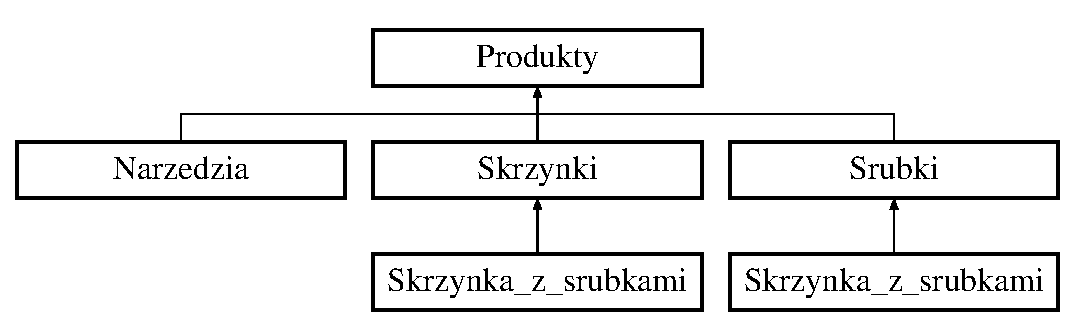
\includegraphics[height=3.000000cm]{class_produkty}
\end{center}
\end{figure}
\subsection*{Public Member Functions}
\begin{DoxyCompactItemize}
\item 
virtual void \mbox{\hyperlink{class_produkty_a720c6591cfbb332f99baccf0f54c4ada}{wypisz}} ()
\item 
void \mbox{\hyperlink{class_produkty_a73fe67e794f741b972330c09a8cf8e55}{Wstaw\+\_\+nazwe\+\_\+cene}} ()
\item 
void \mbox{\hyperlink{class_produkty_ac38af686bb465b62fd499dec9dd6c246}{Wypisz\+\_\+nazwe\+\_\+cene}} ()
\end{DoxyCompactItemize}
\subsection*{Protected Member Functions}
\begin{DoxyCompactItemize}
\item 
virtual void \mbox{\hyperlink{class_produkty_ad69fa64c8984c55fe9b1a2ade607a0ed}{wstaw}} ()
\item 
virtual void \mbox{\hyperlink{class_produkty_a49c2ba4084346df8e7c987b9ec62676e}{zapisz}} (std\+::ostream \&o) const
\end{DoxyCompactItemize}
\subsection*{Protected Attributes}
\begin{DoxyCompactItemize}
\item 
\mbox{\Hypertarget{class_produkty_aafbfed7251061470ba934e02ef902428}\label{class_produkty_aafbfed7251061470ba934e02ef902428}} 
string {\bfseries nazwa}
\item 
\mbox{\Hypertarget{class_produkty_a28eb276dae9d80062d5384be339d87d9}\label{class_produkty_a28eb276dae9d80062d5384be339d87d9}} 
float {\bfseries cena}
\end{DoxyCompactItemize}
\subsection*{Friends}
\begin{DoxyCompactItemize}
\item 
std\+::ostream \& \mbox{\hyperlink{class_produkty_a222d7f697f1aa66b79aefe7163945973}{operator$<$$<$}} (std\+::ostream \&o, \mbox{\hyperlink{class_produkty}{Produkty}} \&p)
\end{DoxyCompactItemize}


\subsection{Detailed Description}
Klasa abstrakcyjna \mbox{\hyperlink{class_produkty}{Produkty}} umozliwiajaca wprowadzanie oraz reprezentacjie czesci danych o nowych produktach 

\subsection{Member Function Documentation}
\mbox{\Hypertarget{class_produkty_ad69fa64c8984c55fe9b1a2ade607a0ed}\label{class_produkty_ad69fa64c8984c55fe9b1a2ade607a0ed}} 
\index{Produkty@{Produkty}!wstaw@{wstaw}}
\index{wstaw@{wstaw}!Produkty@{Produkty}}
\subsubsection{\texorpdfstring{wstaw()}{wstaw()}}
{\footnotesize\ttfamily void Produkty\+::wstaw (\begin{DoxyParamCaption}{ }\end{DoxyParamCaption})\hspace{0.3cm}{\ttfamily [protected]}, {\ttfamily [virtual]}}

metoda wirtualna sluzaca do wprowadzanaia danych z klawiatury 

Reimplemented in \mbox{\hyperlink{class_skrzynki_a764d5064b25a294b3309dc5077a77921}{Skrzynki}}, \mbox{\hyperlink{class_srubki_a129b7fcf23ad1928f196ca255aa66438}{Srubki}}, \mbox{\hyperlink{class_narzedzia_ade1bd4ecf05c894b263791bfcf0f876f}{Narzedzia}}, and \mbox{\hyperlink{class_skrzynka__z__srubkami_a4726c1844080cb96e833cf16e977ecb3}{Skrzynka\+\_\+z\+\_\+srubkami}}.

\mbox{\Hypertarget{class_produkty_a73fe67e794f741b972330c09a8cf8e55}\label{class_produkty_a73fe67e794f741b972330c09a8cf8e55}} 
\index{Produkty@{Produkty}!Wstaw\+\_\+nazwe\+\_\+cene@{Wstaw\+\_\+nazwe\+\_\+cene}}
\index{Wstaw\+\_\+nazwe\+\_\+cene@{Wstaw\+\_\+nazwe\+\_\+cene}!Produkty@{Produkty}}
\subsubsection{\texorpdfstring{Wstaw\+\_\+nazwe\+\_\+cene()}{Wstaw\_nazwe\_cene()}}
{\footnotesize\ttfamily void Produkty\+::\+Wstaw\+\_\+nazwe\+\_\+cene (\begin{DoxyParamCaption}{ }\end{DoxyParamCaption})}

metoda umozliwiajaca wprowadzenie danych o nazwie i cenie \mbox{\Hypertarget{class_produkty_a720c6591cfbb332f99baccf0f54c4ada}\label{class_produkty_a720c6591cfbb332f99baccf0f54c4ada}} 
\index{Produkty@{Produkty}!wypisz@{wypisz}}
\index{wypisz@{wypisz}!Produkty@{Produkty}}
\subsubsection{\texorpdfstring{wypisz()}{wypisz()}}
{\footnotesize\ttfamily void Produkty\+::wypisz (\begin{DoxyParamCaption}{ }\end{DoxyParamCaption})\hspace{0.3cm}{\ttfamily [virtual]}}

metoda wirtualna wypisujaca dane 

Reimplemented in \mbox{\hyperlink{class_skrzynki_adcf60a88ed78fba5a2dfdb54fa82b236}{Skrzynki}}, \mbox{\hyperlink{class_srubki_a0ac1f1ce5748283a13b0f554add73f0b}{Srubki}}, \mbox{\hyperlink{class_narzedzia_a39cd48d9367f3a4e8fcc30878a320338}{Narzedzia}}, and \mbox{\hyperlink{class_skrzynka__z__srubkami_ac543a438ce88bc79a9e8a398b6beff7c}{Skrzynka\+\_\+z\+\_\+srubkami}}.

\mbox{\Hypertarget{class_produkty_ac38af686bb465b62fd499dec9dd6c246}\label{class_produkty_ac38af686bb465b62fd499dec9dd6c246}} 
\index{Produkty@{Produkty}!Wypisz\+\_\+nazwe\+\_\+cene@{Wypisz\+\_\+nazwe\+\_\+cene}}
\index{Wypisz\+\_\+nazwe\+\_\+cene@{Wypisz\+\_\+nazwe\+\_\+cene}!Produkty@{Produkty}}
\subsubsection{\texorpdfstring{Wypisz\+\_\+nazwe\+\_\+cene()}{Wypisz\_nazwe\_cene()}}
{\footnotesize\ttfamily void Produkty\+::\+Wypisz\+\_\+nazwe\+\_\+cene (\begin{DoxyParamCaption}{ }\end{DoxyParamCaption})}

metoda wypisujaca dane o nazwie i cenie \mbox{\Hypertarget{class_produkty_a49c2ba4084346df8e7c987b9ec62676e}\label{class_produkty_a49c2ba4084346df8e7c987b9ec62676e}} 
\index{Produkty@{Produkty}!zapisz@{zapisz}}
\index{zapisz@{zapisz}!Produkty@{Produkty}}
\subsubsection{\texorpdfstring{zapisz()}{zapisz()}}
{\footnotesize\ttfamily void Produkty\+::zapisz (\begin{DoxyParamCaption}\item[{std\+::ostream \&}]{o }\end{DoxyParamCaption}) const\hspace{0.3cm}{\ttfamily [protected]}, {\ttfamily [virtual]}}

metoda zapisujaca dane do pliku wprowadzane podczas dzialania programu 

Reimplemented in \mbox{\hyperlink{class_skrzynki_a2980647e51a17161872064efc5f1b185}{Skrzynki}}, \mbox{\hyperlink{class_srubki_a2d8edbd9d8170f12378c750f634a7ecd}{Srubki}}, \mbox{\hyperlink{class_narzedzia_a4178a26508e00853e8c5c483f9a439a3}{Narzedzia}}, and \mbox{\hyperlink{class_skrzynka__z__srubkami_a62ccdf02cb9d364630ebea27ea94f2a3}{Skrzynka\+\_\+z\+\_\+srubkami}}.



\subsection{Friends And Related Function Documentation}
\mbox{\Hypertarget{class_produkty_a222d7f697f1aa66b79aefe7163945973}\label{class_produkty_a222d7f697f1aa66b79aefe7163945973}} 
\index{Produkty@{Produkty}!operator$<$$<$@{operator$<$$<$}}
\index{operator$<$$<$@{operator$<$$<$}!Produkty@{Produkty}}
\subsubsection{\texorpdfstring{operator$<$$<$}{operator<<}}
{\footnotesize\ttfamily std\+::ostream\& operator$<$$<$ (\begin{DoxyParamCaption}\item[{std\+::ostream \&}]{o,  }\item[{\mbox{\hyperlink{class_produkty}{Produkty}} \&}]{p }\end{DoxyParamCaption})\hspace{0.3cm}{\ttfamily [friend]}}

funkcja zaprzyjazniona stumienia wyjscia umozwiawajaca zapis do pliku 

The documentation for this class was generated from the following files\+:\begin{DoxyCompactItemize}
\item 
Produkty.\+h\item 
Produkty.\+cpp\end{DoxyCompactItemize}

\hypertarget{class_sterowanie}{}\section{Sterowanie Class Reference}
\label{class_sterowanie}\index{Sterowanie@{Sterowanie}}


{\ttfamily \#include $<$Nagłówek.\+h$>$}

\subsection*{Public Member Functions}
\begin{DoxyCompactItemize}
\item 
\mbox{\hyperlink{class_sterowanie_aa583fe9aa2a8cf2ef0bdaef4ff1f63fe}{Sterowanie}} ()
\item 
void \mbox{\hyperlink{class_sterowanie_a6134abccc542aa29b0b0d7c49e252033}{Menu}} ()
\item 
void \mbox{\hyperlink{class_sterowanie_a98e679db65380008ee5c4315bcdea4ff}{Wczytaj}} ()
\item 
void \mbox{\hyperlink{class_sterowanie_a13ce815612492fcc3837c7779def228e}{Wypisz}} ()
\item 
void \mbox{\hyperlink{class_sterowanie_ab11ff3f1364a7b9bb115e927f217f372}{Wypisz\+\_\+narzedzia}} ()
\item 
void \mbox{\hyperlink{class_sterowanie_a2cfe2301e3be2dca7eafb8619a35adb6}{Wypisz\+\_\+srubki}} ()
\item 
void \mbox{\hyperlink{class_sterowanie_a4b0434e74486dfb72bfdc81e93e3c74a}{Wypisz\+\_\+skrzynka}} ()
\item 
void \mbox{\hyperlink{class_sterowanie_a632b8bffe5b03b03564cf3e1aa02dba1}{znajdz}} ()
\item 
void \mbox{\hyperlink{class_sterowanie_aa2c9acc434f34354fe40243b53c295ee}{Zapis\+\_\+do\+\_\+pliku}} ()
\item 
\mbox{\hyperlink{class_sterowanie_ae407297205e8e717b1133762439d8a66}{$\sim$\+Sterowanie}} ()
\end{DoxyCompactItemize}


\subsection{Detailed Description}
Klasa zajmujaca sie sterowaniem calego programu 

\subsection{Constructor \& Destructor Documentation}
\mbox{\Hypertarget{class_sterowanie_aa583fe9aa2a8cf2ef0bdaef4ff1f63fe}\label{class_sterowanie_aa583fe9aa2a8cf2ef0bdaef4ff1f63fe}} 
\index{Sterowanie@{Sterowanie}!Sterowanie@{Sterowanie}}
\index{Sterowanie@{Sterowanie}!Sterowanie@{Sterowanie}}
\subsubsection{\texorpdfstring{Sterowanie()}{Sterowanie()}}
{\footnotesize\ttfamily Sterowanie\+::\+Sterowanie (\begin{DoxyParamCaption}{ }\end{DoxyParamCaption})\hspace{0.3cm}{\ttfamily [inline]}}

Konstruktor ustawiajacy wartosci pol klasy \mbox{\hyperlink{class_sterowanie}{Sterowanie}} \mbox{\Hypertarget{class_sterowanie_ae407297205e8e717b1133762439d8a66}\label{class_sterowanie_ae407297205e8e717b1133762439d8a66}} 
\index{Sterowanie@{Sterowanie}!````~Sterowanie@{$\sim$\+Sterowanie}}
\index{````~Sterowanie@{$\sim$\+Sterowanie}!Sterowanie@{Sterowanie}}
\subsubsection{\texorpdfstring{$\sim$\+Sterowanie()}{~Sterowanie()}}
{\footnotesize\ttfamily Sterowanie\+::$\sim$\+Sterowanie (\begin{DoxyParamCaption}{ }\end{DoxyParamCaption})\hspace{0.3cm}{\ttfamily [inline]}}

Destuktor usuwajacy tablice Produktow 

\subsection{Member Function Documentation}
\mbox{\Hypertarget{class_sterowanie_a6134abccc542aa29b0b0d7c49e252033}\label{class_sterowanie_a6134abccc542aa29b0b0d7c49e252033}} 
\index{Sterowanie@{Sterowanie}!Menu@{Menu}}
\index{Menu@{Menu}!Sterowanie@{Sterowanie}}
\subsubsection{\texorpdfstring{Menu()}{Menu()}}
{\footnotesize\ttfamily void Sterowanie\+::\+Menu (\begin{DoxyParamCaption}{ }\end{DoxyParamCaption})}

Metoda wypisujaca mozliwe opcjie do wyboru w programie przez uzytkownika \mbox{\Hypertarget{class_sterowanie_a98e679db65380008ee5c4315bcdea4ff}\label{class_sterowanie_a98e679db65380008ee5c4315bcdea4ff}} 
\index{Sterowanie@{Sterowanie}!Wczytaj@{Wczytaj}}
\index{Wczytaj@{Wczytaj}!Sterowanie@{Sterowanie}}
\subsubsection{\texorpdfstring{Wczytaj()}{Wczytaj()}}
{\footnotesize\ttfamily void Sterowanie\+::\+Wczytaj (\begin{DoxyParamCaption}{ }\end{DoxyParamCaption})}

Metoda wczytujaca dane produktow podane przez uzytkownika oraz przyporzadkowuje mu odpowiedni obiekt klasy \mbox{\hyperlink{class_kolekcja}{Kolekcja}} gdy tablia produtow jest za mala nastepuje relokacja \mbox{\Hypertarget{class_sterowanie_a13ce815612492fcc3837c7779def228e}\label{class_sterowanie_a13ce815612492fcc3837c7779def228e}} 
\index{Sterowanie@{Sterowanie}!Wypisz@{Wypisz}}
\index{Wypisz@{Wypisz}!Sterowanie@{Sterowanie}}
\subsubsection{\texorpdfstring{Wypisz()}{Wypisz()}}
{\footnotesize\ttfamily void Sterowanie\+::\+Wypisz (\begin{DoxyParamCaption}{ }\end{DoxyParamCaption})}

Metoda wypisujaca informacjie wszystkich produktach \mbox{\Hypertarget{class_sterowanie_ab11ff3f1364a7b9bb115e927f217f372}\label{class_sterowanie_ab11ff3f1364a7b9bb115e927f217f372}} 
\index{Sterowanie@{Sterowanie}!Wypisz\+\_\+narzedzia@{Wypisz\+\_\+narzedzia}}
\index{Wypisz\+\_\+narzedzia@{Wypisz\+\_\+narzedzia}!Sterowanie@{Sterowanie}}
\subsubsection{\texorpdfstring{Wypisz\+\_\+narzedzia()}{Wypisz\_narzedzia()}}
{\footnotesize\ttfamily void Sterowanie\+::\+Wypisz\+\_\+narzedzia (\begin{DoxyParamCaption}{ }\end{DoxyParamCaption})}

Metoda wysisujaca informacjie o wszystkich narzedziach \mbox{\Hypertarget{class_sterowanie_a4b0434e74486dfb72bfdc81e93e3c74a}\label{class_sterowanie_a4b0434e74486dfb72bfdc81e93e3c74a}} 
\index{Sterowanie@{Sterowanie}!Wypisz\+\_\+skrzynka@{Wypisz\+\_\+skrzynka}}
\index{Wypisz\+\_\+skrzynka@{Wypisz\+\_\+skrzynka}!Sterowanie@{Sterowanie}}
\subsubsection{\texorpdfstring{Wypisz\+\_\+skrzynka()}{Wypisz\_skrzynka()}}
{\footnotesize\ttfamily void Sterowanie\+::\+Wypisz\+\_\+skrzynka (\begin{DoxyParamCaption}{ }\end{DoxyParamCaption})}

Metoda wysisujaca informacjie o wszystkich skrzynkach \mbox{\Hypertarget{class_sterowanie_a2cfe2301e3be2dca7eafb8619a35adb6}\label{class_sterowanie_a2cfe2301e3be2dca7eafb8619a35adb6}} 
\index{Sterowanie@{Sterowanie}!Wypisz\+\_\+srubki@{Wypisz\+\_\+srubki}}
\index{Wypisz\+\_\+srubki@{Wypisz\+\_\+srubki}!Sterowanie@{Sterowanie}}
\subsubsection{\texorpdfstring{Wypisz\+\_\+srubki()}{Wypisz\_srubki()}}
{\footnotesize\ttfamily void Sterowanie\+::\+Wypisz\+\_\+srubki (\begin{DoxyParamCaption}{ }\end{DoxyParamCaption})}

Metoda wysisujaca informacjie o wszystkich srubkach \mbox{\Hypertarget{class_sterowanie_aa2c9acc434f34354fe40243b53c295ee}\label{class_sterowanie_aa2c9acc434f34354fe40243b53c295ee}} 
\index{Sterowanie@{Sterowanie}!Zapis\+\_\+do\+\_\+pliku@{Zapis\+\_\+do\+\_\+pliku}}
\index{Zapis\+\_\+do\+\_\+pliku@{Zapis\+\_\+do\+\_\+pliku}!Sterowanie@{Sterowanie}}
\subsubsection{\texorpdfstring{Zapis\+\_\+do\+\_\+pliku()}{Zapis\_do\_pliku()}}
{\footnotesize\ttfamily void Sterowanie\+::\+Zapis\+\_\+do\+\_\+pliku (\begin{DoxyParamCaption}{ }\end{DoxyParamCaption})}

Metoda zapisujaca wprowadzane dane do pliku \mbox{\Hypertarget{class_sterowanie_a632b8bffe5b03b03564cf3e1aa02dba1}\label{class_sterowanie_a632b8bffe5b03b03564cf3e1aa02dba1}} 
\index{Sterowanie@{Sterowanie}!znajdz@{znajdz}}
\index{znajdz@{znajdz}!Sterowanie@{Sterowanie}}
\subsubsection{\texorpdfstring{znajdz()}{znajdz()}}
{\footnotesize\ttfamily void Sterowanie\+::znajdz (\begin{DoxyParamCaption}{ }\end{DoxyParamCaption})}

Metoda znajdujaca po nazwie informacjie o produkcie 

The documentation for this class was generated from the following files\+:\begin{DoxyCompactItemize}
\item 
Nagłówek.\+h\item 
Sterowanie.\+cpp\end{DoxyCompactItemize}

%--- End generated contents ---

% Index
\backmatter
\newpage
\phantomsection
\clearemptydoublepage
\addcontentsline{toc}{chapter}{Index}
\printindex

\end{document}
